\documentclass[landscape,25pt,a0paper,margin=0.75in]{tikzposter}

\usepackage{rubylatex}
\usepackage{amsmath}
\usepackage{listings}
\usepackage{graphicx}
\usepackage{minted}

\usepackage{tikz}
\usetikzlibrary{automata,positioning}


\title{$\RbTeX$}
\institute{Christopher Newport University}
\author{Steven Rosendahl}

\newcommand{\inlinecode}[1]{\texttt{#1}}
\newcommand{\luatex}{\inlinecode{lualatex}\ }
\newcommand{\rbtexc}{\inlinecode{rblatex}\ }

\usetheme{Envelope}

\begin{document}
\maketitle

\begin{columns}

\column{0.25}
\block{Abstract}{
Modern \LaTeX\ distributions include a tool called \luatex that allows users to
dynamically produce content via use of Lua code. Unfortunately, the Lua standard libraries do not
have as much functionality as other popular scripting languages, such as Ruby. The goal of this
project is to incorporate Ruby into \LaTeX\ in a manner similar to \luatex, but with the power and
simplicity of Ruby over Lua.
}

\column{0.5}
\block{Working Examples}{

}

\block{How It Works}{
In order to correctly compile a document using $\RbTeX$, one must run the \rbtexc command on a valid
\LaTeX\ document. The workflow of $\RbTeX$ looks like\\
% \begin{center}
% {%\centering
\resizebox{0.45\textwidth}{!}{%
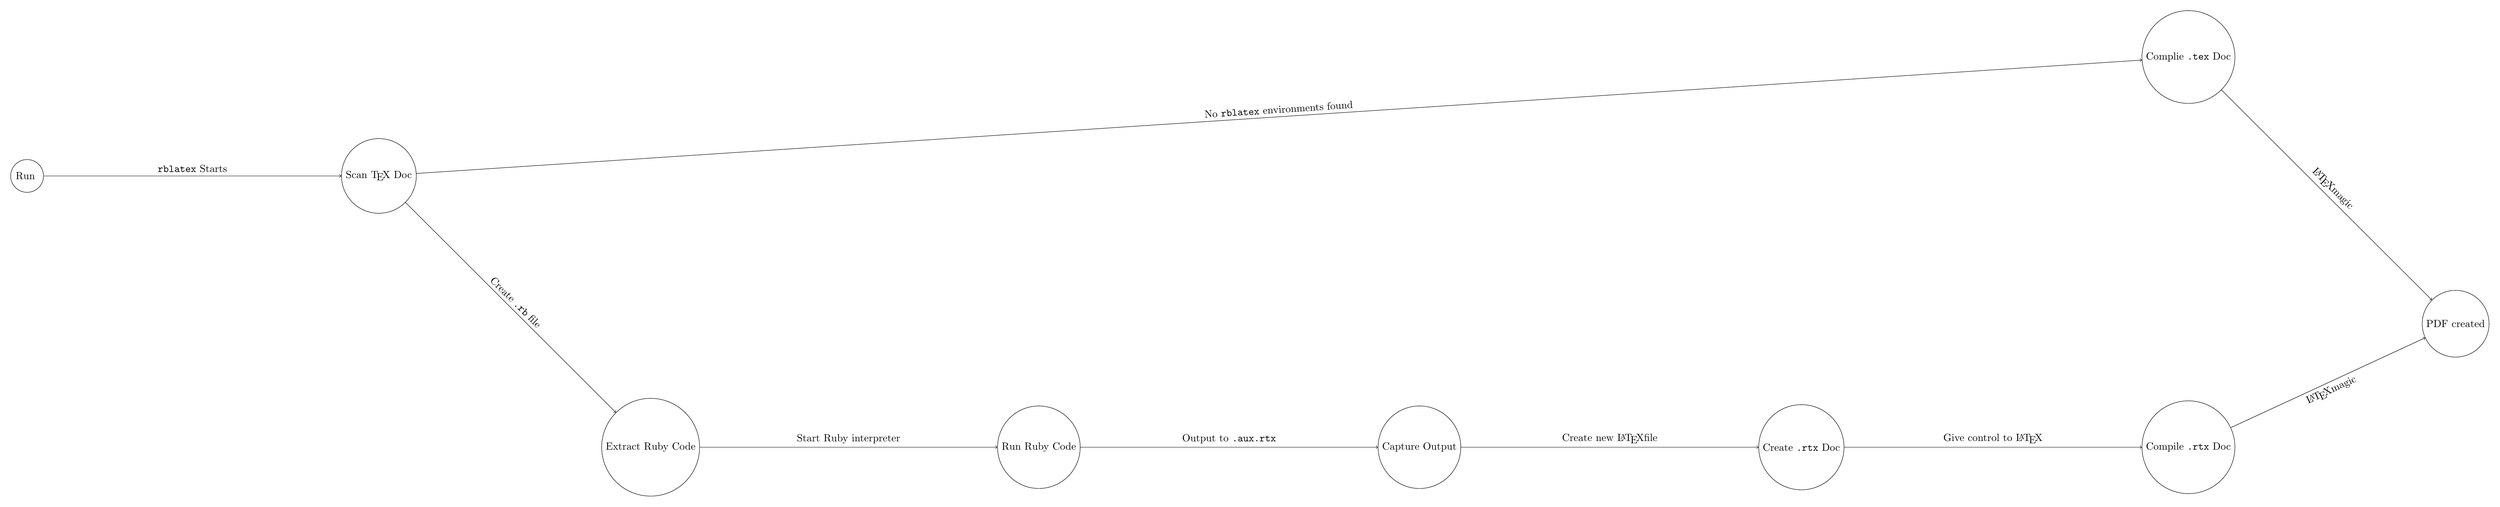
\begin{tikzpicture}%[on grid,auto]

    \node[state] (start) {Run $\RbTeX$};
    \node[state] (scan) [right =10cm of start] {Scan \TeX\ Doc};
    \node[state] (extract) [below right =10cm of scan] {Extract Ruby Code};
    \node[state] (run) [right =10cm of extract] {Run Ruby Code};
    \node[state] (cap) [right =10cm of run] {Capture Output};
    \node[state] (new) [right =10cm of cap] {Create \inlinecode{.rtx} Doc};
    \node[state] (newc) [right =10cm of new]{Compile \inlinecode{.rtx} Doc};
    \node[state] (oldc) [above =10cm of newc]{Complie \inlinecode{.tex} Doc};
    \node[state] (pdf) [below right =10cm of oldc]{PDF created};

    \path[->]
    (start)     edge node [above] {\rbtexc Starts} (scan)
    (scan)      edge node [bend right=45, sloped, above] {Create \inlinecode{.rb} file} (extract)
                edge node [bend right=45, sloped, above] {No \rbtexc environments found} (oldc)
    (extract)   edge node [above] {Start Ruby interpreter} (run)
    (run)       edge node [above] {Output to \inlinecode{.aux.rtx}} (cap)
    (cap)       edge node [above] {Create new \LaTeX file} (new)
    (new)       edge node [above] {Give control to \LaTeX} (newc)
    (newc)      edge node [bend right, sloped, below] {\LaTeX magic} (pdf)
    (oldc)      edge node [bend right, sloped, above] {\LaTeX magic} (pdf);
    % (cap)       edge node [above] {}

\end{tikzpicture}
}
% }
\noindent\\
More text here.
% \end{center}

}

\column{0.25}
\block{}

\end{columns}
\end{document}
